\documentclass [a4paper] {article}
\usepackage[utf8]{inputenc}
\title{Ciencia de datos, práctica 5}
\author{Juan Casado Ballesteros, Samuel García Gonzalez, Iván Anaya Martín}
\usepackage{Sweave}
\begin{document}
\maketitle

\begin{abstract}
Pendiente
\end{abstract}

\newpage

\newpage
\section{K-vecinos sobre la muestra proporcionada para obtener outliers}

Aplicaremos el algoritmo k-vecinos sobre la muestra que tenemos.
Este algoritmo identificará de forma supervisada en la muestra datos anómalos, para poder obtener los outliers.
En primer lugar deberemos cargar esta desde un archivo .txt.
\begin{Schunk}
\begin{Sinput}
> datos1 <- read.table("datos1.txt")
> datos1
\end{Sinput}
\begin{Soutput}
  Teoria Laboratorio
1      4           4
2      4           3
3      5           5
4      1           1
5      5           4
\end{Soutput}
\end{Schunk}

En segundo lugar calculamos las distancias euclídeas entre todos los puntos
\begin{Schunk}
\begin{Sinput}
> distancias <- as.matrix(dist(datos1))
> distancias
\end{Sinput}
\begin{Soutput}
         1        2        3        4        5
1 0.000000 1.000000 1.414214 4.242641 1.000000
2 1.000000 0.000000 2.236068 3.605551 1.414214
3 1.414214 2.236068 0.000000 5.656854 1.000000
4 4.242641 3.605551 5.656854 0.000000 5.000000
5 1.000000 1.414214 1.000000 5.000000 0.000000
\end{Soutput}
\end{Schunk}

Posteriormente, ordenamos las distancias de cada punto a todos los demás.
\begin{Schunk}
\begin{Sinput}
> for(i in 1:length(distanciasordenadas[,1])){
+   distancias[,i] <- sort(distancias[,i])
+ }
> distanciasordenadas <- distancias
\end{Sinput}
\end{Schunk}

Como último paso, reordenamos la matriz para organizarla en función de la distancia
de cada punto a su vecino número 1,2,3...etc. Tras haber organizado la matriz, buscamos en el tercer
vecino, que es el valor k que hemos usado en nuestro análisis para poder identificar los outliers.
\begin{Schunk}
\begin{Sinput}
> outliers_kvecinos = list()
> for(i in 1:length(distanciasordenadas[,1])){
+   if(distanciasordenadas[4,i]>2.5){
+     outliers_kvecinos[[length(outliers_kvecinos)+1]] <- datos1[i,]
+   }
+ }
> outliers_kvecinos
\end{Sinput}
\begin{Soutput}
[[1]]
  Teoria Laboratorio
4      1           1
\end{Soutput}
\end{Schunk}



\section{Deteccion de datos anómalos sobre la resistencia }

\begin{Schunk}
\begin{Sinput}
> datos2 <- read.table("datos2.txt")
> datos2 <- data.frame(datos2)
> datos2
\end{Sinput}
\begin{Soutput}
  Resistencia Densidad
1         3.0      2.0
2         3.5     12.0
3         4.7      4.1
4         5.2      4.9
5         7.1      6.1
6         6.2      5.2
7        14.0      5.3
\end{Soutput}
\end{Schunk}

Cargamos los datos de la densidad y la resistencia de un txt

\begin{center}
\begin{Schunk}
\begin{Sinput}
> boxplot(datos2$Resistencia, range=1.5, horizontal = TRUE)
\end{Sinput}
\end{Schunk}
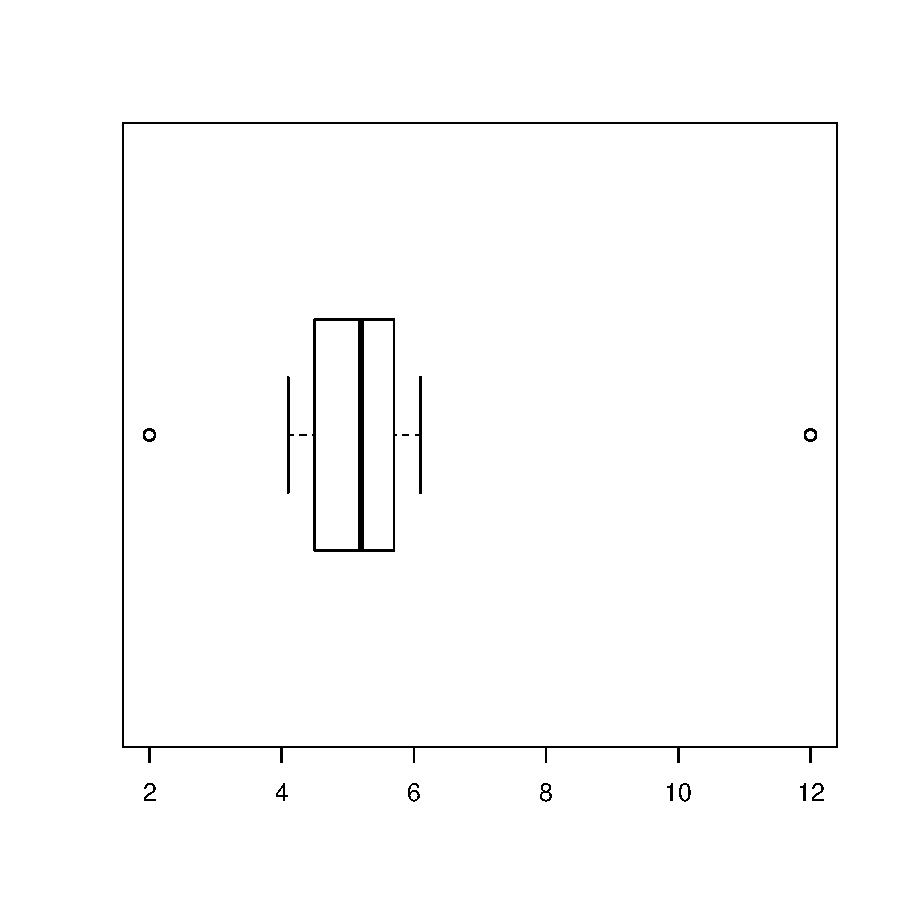
\includegraphics{entrega-plot_caja_bigotes}
\end{center}


Usamos la funcion para ver los datos en una caja de bigotes. 

\begin{center}
\begin{Schunk}
\begin{Sinput}
> cuart1_res<-quantile(datos2$Resistencia,0.25)
> cuart3_res<-quantile(datos2$Resistencia,0.75)
> int=c(cuart1_res-1.5*(cuart3_res-cuart1_res), cuart3_res+1.5*(cuart3_res-cuart1_res))
> outliers_cuartiles_resistencia = list()
> for(i in 1:length(datos2$Resistencia)){
+   if(datos2$Resistencia[i]<int[1]||datos2$Resistencia[i]>int[2]){
+     outliers_cuartiles_resistencia[[length(outliers_cuartiles_resistencia)+1]] <- t(matrix(c(i, datos2[i,]$Resistencia), dimnames=list(c("Indice","Resistencia"))))
+   }
+ }
> outliers_cuartiles_resistencia
\end{Sinput}
\begin{Soutput}
[[1]]
     Indice Resistencia
[1,]      7          14
\end{Soutput}
\end{Schunk}
\end{center}

Mediante el calculo de los primer cuartil y del tercero aplicamos la formula para ver si existe algun outlier en la muestra.
 Esto nos da un rango todo los valores fuera de este rango son outlier. Luego comprobamos todo los valores de los datos para 
 comprobar si existe, y por lo tanto mostramos. 

 Como vemos el valor 12 es un outlier de los datos

\begin{center}
\begin{Schunk}
\begin{Sinput}
> boxplot(datos2$Densidad, range=1.5, horizontal = TRUE)
\end{Sinput}
\end{Schunk}
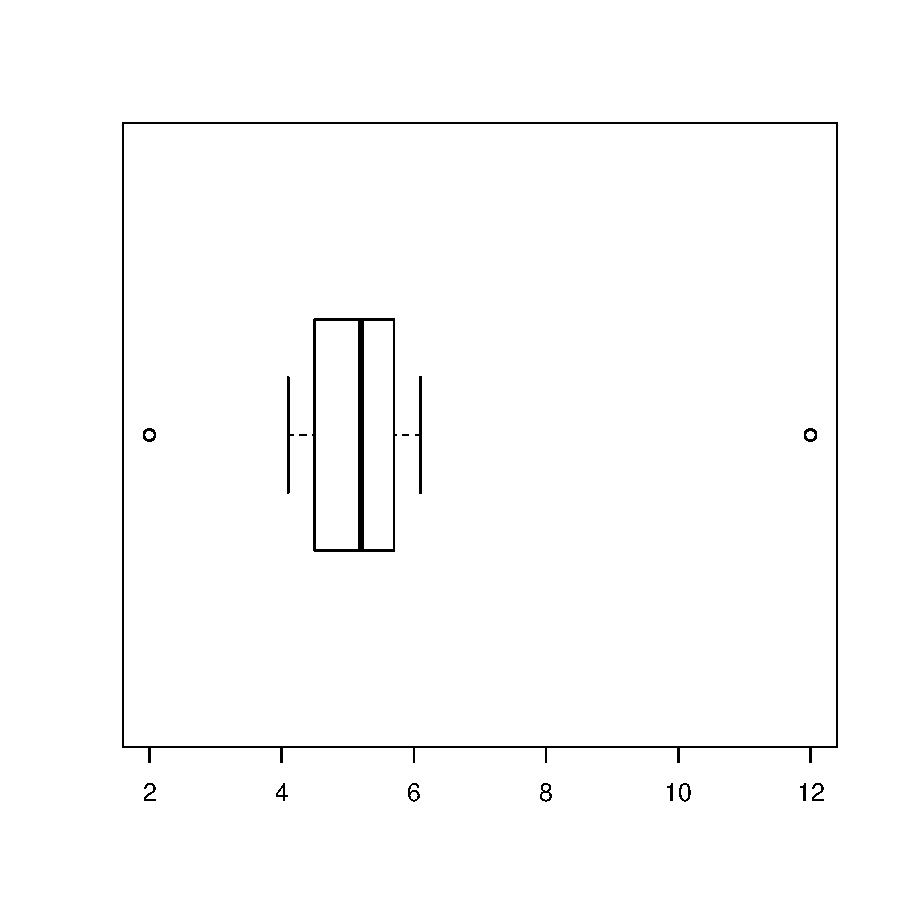
\includegraphics{entrega-plot_caja_bigotes}
\end{center}


\begin{center}
\begin{Schunk}
\begin{Sinput}
> cuart1_den<-quantile(datos2$Densidad,0.25)
> cuart3_den<-quantile(datos2$Densidad,0.75)
> int=c(cuart1_den-1.5*(cuart3_den-cuart1_den), cuart3_den+1.5*(cuart3_den-cuart1_den))
> outliers_cuartiles_densidad <- list()
> for(i in 1:length(datos2$Densidad)){
+   if(datos2$Densidad[i]<int[1]||datos2$Densidad[i]>int[2]){
+     outliers_cuartiles_densidad[[length(outliers_cuartiles_densidad)+1]] <- t(matrix(c(i, datos2[i,]$Densidad), dimnames=list(c("Indice","Densidad"))))
+   }
+ }
> outliers_cuartiles_densidad
\end{Sinput}
\begin{Soutput}
[[1]]
     Indice Densidad
[1,]      1        2

[[2]]
     Indice Densidad
[1,]      2       12
\end{Soutput}
\end{Schunk}
\end{center}

Realizamos, vemos que esta vez hay dos outlier uno es el 2 y el otro 12 de la densidad 


\newpage
\section{Dispersión sobre la densidad, desviación típica}

\begin{Schunk}
\begin{Sinput}
> datos2 <- read.table("datos2.txt")
\end{Sinput}
\end{Schunk}

\begin{center}
\begin{Schunk}
\begin{Sinput}
> plotFrecuencyData(datos2$Densidad)
\end{Sinput}
\end{Schunk}
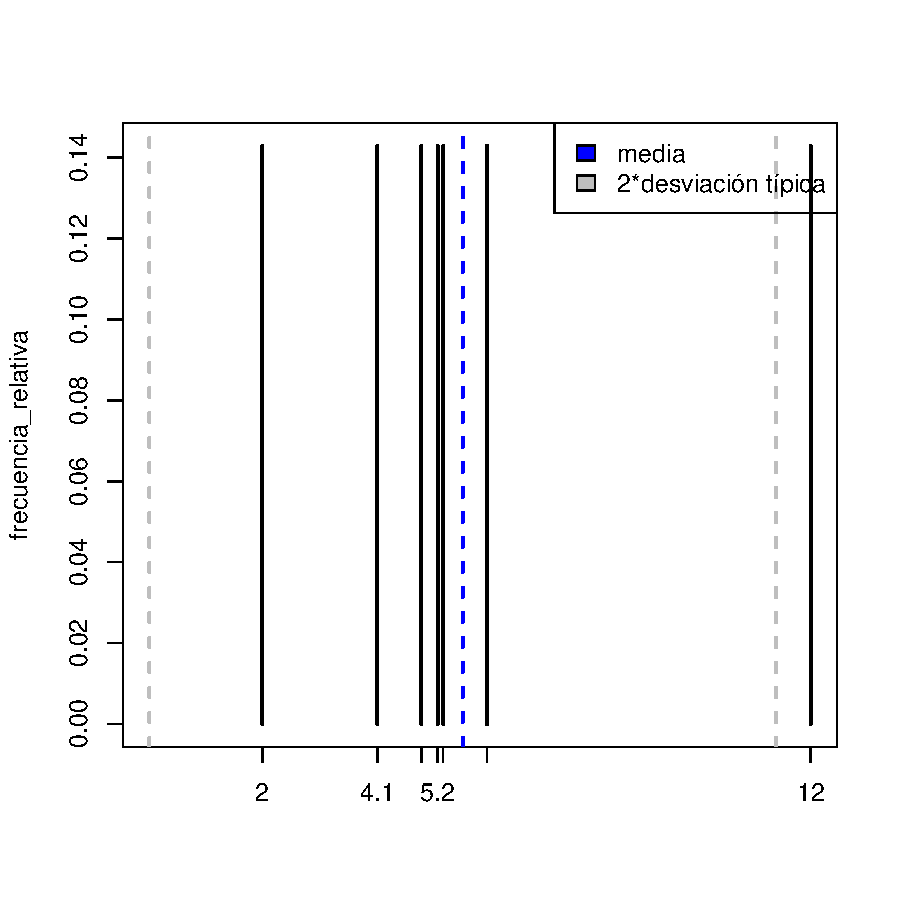
\includegraphics{entrega-desviacion_tipica_densidad_plot}
\end{center}
\begin{Schunk}
\begin{Sinput}
> int <- c(mediaAritmetica(datos2$Densidad) - 2*desviacionTipica(datos2$Densidad), mediaAritmetica(datos2$Densidad) + 2*desviacionTipica(datos2$Densidad))
> outliers_desviacion = list()
> for(i in 1:length(datos2$Densidad)) {
+   if ((datos2$Densidad[i]<int[1]) || (datos2$Densidad[i]>int[2])) {
+     outliers_desviacion[[length(outliers_desviacion)+1]] <- t(matrix(c(i, datos2[i,]$Densidad), dimnames=list(c("Indice","Densidad"))))
+   }
+ }
> outliers_desviacion
\end{Sinput}
\begin{Soutput}
[[1]]
     Indice Densidad
[1,]      2       12
\end{Soutput}
\end{Schunk}

\begin{center}
\begin{Schunk}
\begin{Sinput}
> plotFrecuencyData(datos2$Resistencia)
\end{Sinput}
\end{Schunk}
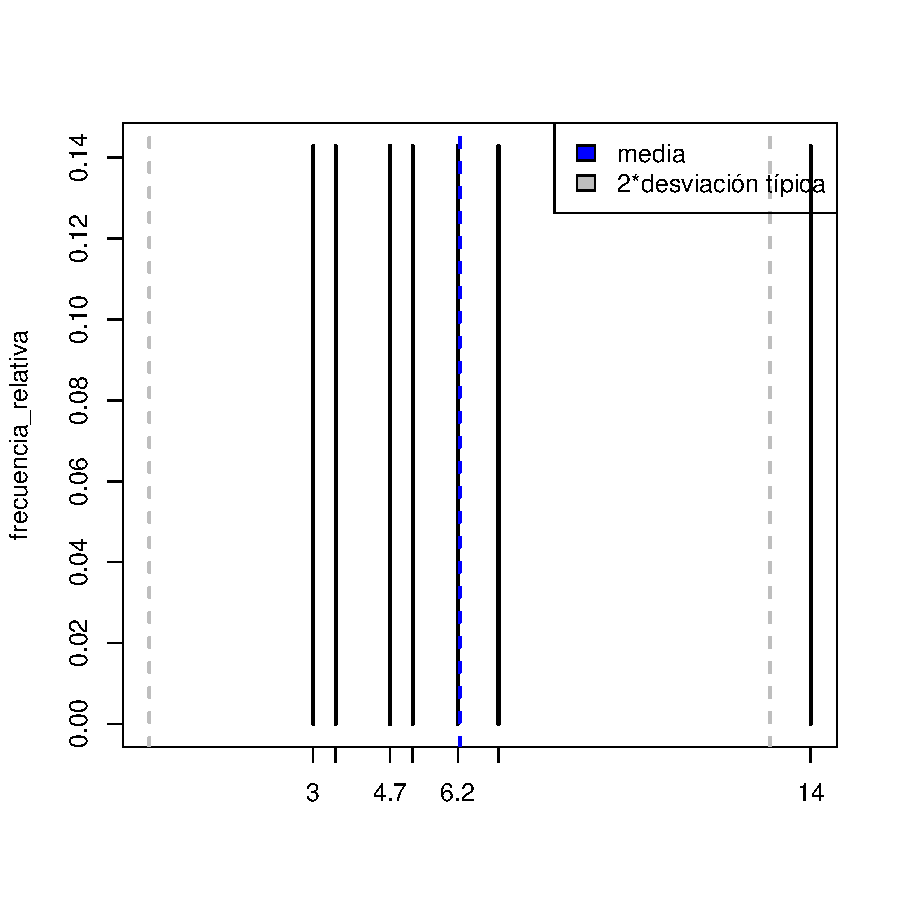
\includegraphics{entrega-desviacion_tipica_resistencia_plot}
\end{center}
\begin{Schunk}
\begin{Sinput}
> int <- c(mediaAritmetica(datos2$Resistencia) - 2*desviacionTipica(datos2$Resistencia), mediaAritmetica(datos2$Resistencia) + 2*desviacionTipica(datos2$Resistencia))
> outliers_desviacion = list()
> for(i in 1:length(datos2$Resistencia)) {
+   if ((datos2$Resistencia[i]<int[1]) || (datos2$Resistencia[i]>int[2])) {
+     outliers_desviacion[[length(outliers_desviacion)+1]] <- t(matrix(c(i, datos2[i,]$Resistencia), dimnames=list(c("Indice","Resistencia"))))
+   }
+ }
> outliers_desviacion
\end{Sinput}
\begin{Soutput}
[[1]]
     Indice Resistencia
[1,]      7          14
\end{Soutput}
\end{Schunk}

\section{detección de datos anómalos sobre la regresión de la densidad en función de la resistencia}

En este análisis detectamos los outliers utilizando la recta de regresión y
el error estándar de los residuos. Como primer paso leemos la tabla de los datos.
\begin{Schunk}
\begin{Sinput}
> datos2 <- read.table("datos2.txt")
> datos2
\end{Sinput}
\begin{Soutput}
  Resistencia Densidad
1         3.0      2.0
2         3.5     12.0
3         4.7      4.1
4         5.2      4.9
5         7.1      6.1
6         6.2      5.2
7        14.0      5.3
\end{Soutput}
\end{Schunk}
Seguidamente calculamos la recta de regresión sobre los datos.
\begin{Schunk}
\begin{Sinput}
> dFr=lm(datos2$Densidad~datos2$Resistencia)
\end{Sinput}
\end{Schunk}
Posteriormente, obtenemos los residuos calculados a partir de la recta de regresión.
\begin{Schunk}
\begin{Sinput}
> res=summary(dFr)$residuals
\end{Sinput}
\end{Schunk}
Para finalizar, calculamos el error estándar de los residuos, y a partir de él comparamos cada
uno para comprobar si algún residuo es 2 veces mayor que el error estándar. Si se da el caso, 
podemos considerar ese punto como un outlier. 
\begin{Schunk}
\begin{Sinput}
> sr=sqrt(sum(res^2)/length(res))
> outliers_regresion = list()
> for(i in 1:length(res)){
+   if(abs(res[i])>2*sr){
+     outliers_regresion[[length(outliers_regresion)+1]] <- datos2[i,]
+   }
+ }
> outliers_regresion
\end{Sinput}
\begin{Soutput}
[[1]]
  Resistencia Densidad
2         3.5       12
\end{Soutput}
\end{Schunk}

\end{document}
